%--------------------------------------------------------------------
%  Capítulo 4 — Desarrollo del Proyecto
%--------------------------------------------------------------------
\chapter{Desarrollo del Proyecto}
\label{chap:desarrollo}
\justifying

En este capítulo se detalla el proceso de desarrollo de \textbf{Tutor Virtual}, desde la concepción inicial y la configuración del entorno de trabajo hasta la implementación del prototipo funcional.

La metodología de desarrollo se ha basado en un enfoque iterativo e incremental, reflejado en la estructura de este capítulo, que se organiza en etapas. Cada etapa aborda aspectos específicos del sistema, incluyendo la definición de requisitos, la selección tecnológica, el diseño de la arquitectura, la implementación de la base de datos, el desarrollo del backend y del frontend, y finalmente, la integración de todas las capas del sistema.

%--------------------------------------------------------------------
\section{Fase Inicial: Planificación y Diseño del Entorno}
\label{sec:desarrollo_entorno}

La construcción de \textbf{Tutor Virtual} comenzó con una fase de planificación. Esta etapa incluyó tres actividades principales: (i) la definición y priorización de requisitos funcionales y no funcionales; (ii) un análisis comparativo de las herramientas y tecnologías a emplear; y (iii) el diseño de una arquitectura de directorios y componentes que promoviera la modularidad y la \emph{separación de conceptos}.

%====================================================================
\subsection{Definición y Priorización de Requisitos}
\label{ssec:desarrollo_reqs}

\paragraph{Metodología de Recopilación y Priorización.}
Dada la naturaleza del proyecto y las limitaciones de tiempo y recursos, la fase de toma de requisitos fue llevada a cabo por el propio desarrollador, partiendo de la idea inicial del tutor virtual.

Para estructurar y priorizar los requisitos identificados, se empleó la técnica MoSCoW, que clasifica cada requisito como \textbf{M}ust-have (imprescindible), \textbf{S}hould-have (debería tener), \textbf{C}ould-have (podría tener), o \textbf{W}on't-have (no tendrá en esta iteración). Los resultados de esta clasificación se presentan en la Tabla~\ref{tab:desarrollo_reqs}.

\begin{table}[H]
\centering
\begin{tabular}{@{}p{7.5cm}lc@{}}
\toprule
\textbf{Requisito} & \textbf{Tipo} & \textbf{Prioridad (MoSCoW)}\\
\midrule
R1. Gestión de usuarios: Registro, inicio de sesión (login) y autenticación basada en JWT. & F & M \\
R2. Gestión académica: Listar cursos y asignaturas; permitir la inscripción (enrolamiento) del estudiante. & F & M \\
R3. Generación de contenido: Creación de ejercicios con niveles de dificultad graduados (\emph{fácil, intermedio, difícil}). & F & M \\
R4. Interacción y retroalimentación: Proporcionar feedback inmediato a las respuestas del estudiante, incluyendo explicaciones paso a paso. & F & M \\
R5. Seguimiento del estudiante: Panel de progreso individualizado para el estudiante. & F & S \\
R6. Administración del sistema: Interfaz CRUD (Crear, Leer, Actualizar, Borrar) para la gestión de cursos, asignaturas y temas por parte de un administrador. & F & S \\
R7. Funcionamiento \emph{offline-first}: Capacidad del motor de IA para operar localmente sin conexión a internet. & NF & M \\
R8. Rendimiento: Latencia interactiva (\(\le\)\SI{1.5}{s}) en la conversación y generación de ejercicios. & NF & S \\
R9. Mantenimiento: Backups diarios automatizados de la base de datos. & NF & C \\
\bottomrule
\end{tabular}
\caption{Requisitos funcionales (F) y no funcionales (NF) del proyecto Tutor Virtual, priorizados según la técnica MoSCoW.}
\label{tab:desarrollo_reqs}
\end{table}

%====================================================================
\subsection{Análisis y Selección de Herramientas y Tecnologías}
\label{ssec:desarrollo_tooling}

La selección tecnológica se basó en criterios de madurez, comunidad, rendimiento, facilidad de desarrollo y alineación con los requisitos del proyecto. A continuación, se describen las principales herramientas y tecnologías elegidas:

\begin{itemize}[leftmargin=*]
  \item \textbf{Control de Versiones (Git \& GitHub):} Se utilizó un repositorio Git privado en GitHub con un flujo de trabajo basado en una rama permanente: \texttt{main} (para versiones estables). Las nuevas funcionalidades se desarrollaron en ramas \texttt{feature/*} y se integraron mediante \emph{Pull Requests} (PR).

  \item \textbf{Backend (FastAPI):} Se eligió FastAPI por su alto rendimiento (comparable o superior a Node.js y Go para ciertas cargas, gracias a ASGI con Uvicorn y Uvloop), su sistema de tipado basado en Pydantic V2 (que reduce errores y mejora la mantenibilidad), y la generación automática de documentación OpenAPI (Swagger UI y ReDoc). La versión de Python se fijó a \texttt{3.11.11}.

  \item \textbf{Gestión de Migraciones de Base de Datos (Alembic):} Para manejar los cambios en el esquema de la base de datos de forma controlada y versionada, se utilizó Alembic. Cada modificación en los modelos SQLAlchemy generó un script de migración con marca de tiempo (ej. \texttt{alembic revision --autogenerate -m "descripcion\_del\_cambio"}). Esto permite:
        \begin{itemize}
          \item Actualizar (\emph{upgrade}) o revertir (\emph{downgrade}) el esquema de la base de datos en entornos de desarrollo, pruebas (\emph{staging}) y producción.
          \item Mantener un historial completo de cambios en el directorio
          
          \texttt{migrations/versions/}.
          \item Evitar el problema de “\emph{snowflake DB}” (bases de datos con esquemas únicos y difíciles de replicar), permitiendo clonar la estructura exacta de la base de datos en cualquier máquina mediante \texttt{alembic upgrade head}.
        \end{itemize}

  \item \textbf{Base de Datos (PostgreSQL):} Se seleccionó PostgreSQL por su robustez, fiabilidad y amplio conjunto de características SQL estándar y avanzadas. La administración gráfica se realizó con PGAdmin 4.

  \item \textbf{Frontend (React 18 + Vite):} Para la interfaz de usuario, se optó por React 18 debido a su madurez, ecosistema y componentes. Como herramienta de construcción y servidor de desarrollo, se eligió Vite por su velocidad (Hot Module Replacement - HMR típicamente \(<\SI{100}{ms}\)). El estado remoto (comunicación con la API) se gestionó con React Query por sus capacidades de caching, sincronización en segundo plano y optimización de peticiones. Tailwind CSS se utilizó como framework CSS utilitario para un desarrollo ágil y personalizable de la interfaz.

  \item \textbf{Infraestructura de Inteligencia Artificial (llama.cpp + RAG con OpenWebUI en Docker):}
        \begin{description}[leftmargin=*]
          \item[Modelo LLM:] Se seleccionó una versión cuantizada del modelo \texttt{Llama-3 8B} (específicamente, \texttt{llama-3-8B-int4.gguf}, con un tamaño de aproximadamente 7 GB) para permitir su ejecución en hardware de consumo.
          \item[Motor de Inferencia y RAG:] Se utilizó \texttt{llama.cpp} para la inferencia eficiente del modelo en CPU. Para la funcionalidad de Recuperación Aumentada por Generación (RAG), se integró OpenWebUI\footnote{Disponible en \url{https://github.com/open-webui/open-webui}}. OpenWebUI actúa como una puerta de enlace que ingiere documentos (ej. \texttt{numerosNaturales.txt}), los vectoriza utilizando un modelo de embeddings como \texttt{sentence-transformers/all-MiniLM-L6-v2}, y gestiona las consultas semánticas antes de invocar al LLM para generar la respuesta final.
          \item[Contenerización (Docker):] El componente de IA (incluyendo OpenWebUI, llama.cpp y el modelo) fue la única pieza del sistema completamente contenerizada de forma obligatoria. Esto se hizo para cumplir el requisito R7 de aislamiento y despliegue simplificado del motor de IA, mientras que el backend y frontend podían ejecutarse nativamente durante el desarrollo si se deseaba.
        \end{description}
\end{itemize}

La Tabla~\ref{tab:desarrollo_match-tech-require} resume cómo las tecnologías seleccionadas cubren los requisitos clave del proyecto.

\begin{table}[H]
  \centering
  \begin{tabularx}{\linewidth}{@{} l l X @{}}
    \toprule
    \textbf{Tecnología/Herramienta} & \textbf{Requisito(s) Clave} & \textbf{Justificación Principal de la Elección} \\
    \midrule
    FastAPI (Python)     & R1, R2, R6    & Desarrollo rápido de APIs, tipado estricto, rendimiento asíncrono, OpenAPI. \\
    React + Vite         & R2–R6         & Ecosistema maduro, desarrollo basado en componentes, HMR rápido. \\
    React Query          & R3–R5         & Gestión eficiente del estado del servidor, caching, optimización de peticiones. \\
    llama.cpp (local)    & R3, R4, R7    & Permite inferencia de LLM offline, control sobre el modelo. \\
    OpenWebUI (RAG)      & R3, R4        & Facilita la integración de RAG con corpus documental propio. \\
    Docker (para IA)     & R7            & Aísla dependencias complejas de IA, facilita despliegue del motor. \\
    Alembic              & R2, R6        & Gestión segura y versionada de migraciones de esquema de BD. \\
    PostgreSQL           & R1–R6         & Base de datos relacional robusta y estándar. \\
    Git \& GitHub Actions& Todos         & Control de versiones, colaboración, CI/CD para calidad de código. \\
    \bottomrule
  \end{tabularx}
  \caption{Mapeo entre requisitos y tecnologías seleccionadas.}
  \label{tab:desarrollo_match-tech-require}
\end{table}

%====================================================================
\subsection{Diseño de la Arquitectura de Directorios}
\label{ssec:desarrollo_arch}

El proyecto se estructuró en \textbf{dos directorios raíz principales}: \texttt{tutor-backend} y \texttt{tutor-frontend}. Esta separación física, inspirada en principios de arquitecturas limpias (\emph{Clean Architecture}) y microservicios (aunque no estrictamente un microservicio), ofrece varias ventajas:
\begin{enumerate}[leftmargin=*]
  \item \textbf{Despliegue independiente:} Permite desplegar el frontend en un servicio de hosting estático (ej. Netlify, Vercel, GitHub Pages) sin necesidad de un servidor Python, y el backend en una plataforma de aplicaciones (ej. Heroku, Docker en un VPS).
  \item \textbf{Pruebas aisladas:} Facilita la ejecución de pruebas del backend (\texttt{pytest}) sin necesidad de compilar o levantar el entorno de frontend (Node.js, Vite), y viceversa.
  \item \textbf{Pipelines de CI/CD diferenciados:} Posibilita la gestión de pipelines de integración y despliegue continuo distintos para cada parte (ej. construcción de imagen Docker para el backend, \emph{build} estático para el frontend).
  \item \textbf{Equipos especializados (escalabilidad humana):} En un equipo más grande, permitiría que los desarrolladores backend y frontend trabajen en paralelo con menor interferencia.
\end{enumerate}

%------------------------------------------------
\subsubsection*{Estructura del Backend (\texttt{tutor-backend})}
\label{sssec:desarrollo_arch_backend}

La organización de directorios del backend se inspira en patrones de diseño como la arquitectura hexagonal o la arquitectura por capas, buscando una alta cohesión y bajo acoplamiento:

\begin{description}[leftmargin=*,style=unboxed,font=\normalfont]
  \item[\texttt{src/api/}] Contiene los módulos relacionados con la capa de presentación de la API:
    \begin{itemize}
        \item \texttt{routes/}: Define los \emph{routers} de FastAPI para cada conjunto de endpoints (ej. \texttt{auth.py}, \texttt{courses.py}).
        \item \texttt{dependencies/}: Módulos para la inyección de dependencias en FastAPI (ej. obtención de usuario actual, sesión de BD).
        \item \texttt{middlewares/}: Middlewares personalizados (ej. para logging de peticiones, gestión de CORS).
        \item \texttt{schemas/}: Modelos Pydantic para la validación de datos de entrada y serialización de datos de salida.
    \end{itemize}
  \item[\texttt{src/core/}] Almacena la configuración central de la aplicación y utilidades transversales:
    \begin{itemize}
        \item \texttt{config.py}: Carga y gestión de variables de entorno y configuraciones usando Pydantic Settings.
        \item \texttt{security.py}: Funciones para hashing de contraseñas, creación y verificación de JWTs.
        \item \texttt{logging.py}: Configuración del sistema de logging.
    \end{itemize}
  \item[\texttt{src/database/}] Responsable de la interacción con la base de datos:
    \begin{itemize}
        \item \texttt{session.py}: Creación del motor SQLAlchemy, gestión de sesiones de base de datos (incluyendo la dependencia \texttt{get\_db} para FastAPI).
        \item \texttt{base.py}: Declaración de la base para los modelos SQLAlchemy.
    \end{itemize}
  \item[\texttt{src/models/}] Define los modelos ORM de SQLAlchemy que mapean a las tablas de la base de datos (ej. \texttt{user.py}, \texttt{course.py}).
  \item[\texttt{src/services/}] Contiene la lógica de negocio o de dominio de la aplicación. Estos servicios son invocados por los endpoints de la API y operan sobre los modelos (ej. \texttt{user\_service.py}, \texttt{exercise\_service.py}).
  \item[\texttt{src/utils/}] Módulos con funciones de utilidad genéricas y transversales (ej. cliente para Ollama, funciones para normalizar texto, etc.).
  \item[\texttt{migrations/}] Directorio gestionado por Alembic para los scripts de migración de la base de datos.
    \begin{itemize}
        \item \texttt{versions/}: Contiene los scripts de migración individuales.
    \end{itemize}
  \item[\texttt{tests/}] Pruebas automatizadas, divididas en:
    \begin{itemize}
        \item \texttt{unit/}: Pruebas unitarias para componentes aislados (servicios, utils).
        \item \texttt{integration/}: Pruebas de integración que verifican la interacción entre varios componentes (ej. endpoints de API con la base de datos mockeada).
    \end{itemize}
\end{description}

%------------------------------------------------
\subsubsection*{Estructura del Frontend (\texttt{tutor-frontend})}
\label{sssec:desarrollo_arch_frontend}

El frontend sigue una jerarquía inspirada en \emph{Atomic Design} y organizada por características (\emph{feature-based}), promoviendo la reutilización y la claridad:

\begin{description}[leftmargin=*,style=unboxed,font=\normalfont]
  \item[\texttt{src/app/}] Configuración principal de la aplicación React:
    \begin{itemize}
        \item \texttt{App.tsx}: Componente raíz de la aplicación.
        \item \texttt{main.tsx}: Punto de entrada de la aplicación, renderiza \texttt{App}.
        \item \texttt{routes.tsx}: Definición de las rutas de la aplicación utilizando React Router.
        \item \texttt{guards/}: Componentes de guarda para proteger rutas (ej. \texttt{PrivateRoute}, \texttt{AdminRoute}).
    \end{itemize}
  \item[\texttt{src/components/}] Componentes UI reutilizables, organizados por complejidad (Atomic Design):
    \begin{itemize}
        \item \texttt{atoms/}: Los bloques de construcción más pequeños (ej. \texttt{Button.tsx}, \texttt{Spinner.tsx}, \texttt{Input.tsx}). El componente \texttt{MultiCheckList}.
        \item \texttt{molecules/}: Combinaciones de átomos que forman componentes más complejos (ej. \texttt{SearchField.tsx} (input + botón), \texttt{StepIndicator.tsx}).
        \item \texttt{organisms/}: Secciones más grandes de la interfaz compuestas por moléculas y/o átomos (ej. \texttt{NavBar.tsx}, \texttt{Footer.tsx}, \texttt{CrudModal.tsx}).
    \end{itemize}
  \item[\texttt{src/context/}] Proveedores de Contexto de React para la gestión de estado global (ej. \texttt{AuthContext.tsx}, \texttt{ThemeContext.tsx}, \texttt{ViewModeContext.tsx}).
  \item[\texttt{src/features/}] Directorios que encapsulan toda la lógica, componentes específicos, hooks y páginas para una funcionalidad o dominio particular de la aplicación. Esto mejora la localización del código relacionado con una característica:
    \begin{itemize}
        \item \texttt{admin/}: Todo lo relacionado con el panel de administración.
        \item \texttt{auth/}: Páginas de login, registro, hooks de autenticación.
        \item \texttt{dashboard/}: Panel principal del estudiante.
        \item \texttt{explore/}: Funcionalidad para explorar y matricularse en cursos.
        \item \texttt{study/}: Interfaz de estudio y realización de ejercicios.
        \item \texttt{stats/}: Visualización de estadísticas de progreso.
    \end{itemize}
  \item[\texttt{src/hooks/}] Hooks personalizados de React reutilizables en varias características (si no son específicos de una sola feature).
  \item[\texttt{src/services/}] Lógica para interactuar con APIs externas o el backend:
    \begin{itemize}
        \item \texttt{apiClient.ts}: Configuración de Axios o cliente HTTP, incluyendo interceptores.
        \item Lógica específica para consumir los endpoints del backend (ej. \texttt{courseService.ts}). Estos servicios son luego utilizados por React Query hooks.
    \end{itemize}
  \item[\texttt{src/styles/}] Archivos de estilos globales, configuración de Tailwind CSS, variables CSS, etc.
  \item[\texttt{src/types/}] Definiciones de tipos TypeScript compartidas en la aplicación (ej. DTOs para datos de la API, tipos de modelos del frontend).
  \item[\texttt{src/utils/}] Funciones de utilidad genéricas para el frontend.
  \item[\texttt{vite.config.ts}] Archivo de configuración de Vite.
\end{description}

El Listado~\ref{lst:desarrollo_tree-root} presenta una simplificación de la estructura de directorios inicial del monorepo (considerando los dos directorios raíz). La Figura~\ref{fig:desarrollo_folder-layers} ilustra conceptualmente las dependencias entre estas capas.

\begin{lstlisting}[language=bash,caption={Estructura de directorios raíz simplificada del proyecto (snapshot inicial, commit 0d7fe1).},label={lst:desarrollo_tree-root},basicstyle=\fontsize{8}{9.5}\ttfamily]
tutor-virtual/                 # Raíz del proyecto (puede ser un monorepo o dos repos separados)
├── tutor-backend/             # Servicio Backend (FastAPI)
│   ├── src/
│   │   ├── api/               # Endpoints, dependencias, middlewares, schemas Pydantic
│   │   │   ├── dependencies/
│   │   │   ├── middlewares/
│   │   │   ├── routes/
│   │   │   └── schemas/
│   │   ├── core/              # Configuración global, seguridad (JWT, hashing)
│   │   ├── database/          # Configuración de BD (engine, session factory)
│   │   ├── models/            # Modelos ORM SQLAlchemy
│   │   ├── services/          # Lógica de negocio y dominio
│   │   └── utils/             # Funciones de utilidad del backend
│   ├── migrations/            # Scripts de Alembic para migraciones de BD
│   │   └── versions/          # Versiones específicas de migración
│   ├── tests/                 # Pruebas (unitarias y de integración)
│   │   ├── integration/
│   │   └── unit/
│   ├── alembic.ini            # Configuración de Alembic
│   ├── pyproject.toml         # O requirements.txt / Pipfile para dependencias Python
│   └── .env.example           # Ejemplo de variables de entorno
│
└── tutor-frontend/            # Cliente Frontend (React + Vite)
    ├── src/
    │   ├── app/               # Configuración principal de la App (rutas, guards)
    │   ├── components/        # Componentes UI reutilizables (atoms, molecules, organisms)
    │   │   ├── atoms/
    │   │   ├── molecules/
    │   │   └── organisms/
    │   ├── context/           # React Context Providers (auth, theme)
    │   ├── features/          # Módulos por funcionalidad (auth, admin, dashboard, etc.)
    │   │   ├── admin/
    │   │   ├── auth/
    │   │   └── ...
    │   ├── hooks/             # Hooks de React personalizados y reutilizables
    │   ├── services/          # Lógica de cliente API (ej. cliente Axios, funciones de servicio)
    │   ├── styles/            # Estilos globales, config. TailwindCSS
    │   └── types/             # Definiciones TypeScript
    ├── public/                # Activos estáticos
    ├── index.html             # Punto de entrada HTML para Vite
    ├── vite.config.ts         # Configuración de Vite
    ├── tsconfig.json          # Configuración de TypeScript
    ├── package.json           # Dependencias y scripts de Node.js
    └── .env.example           # Ejemplo de variables de entorno para el frontend
\end{lstlisting}

Principios característicos de esta organización:
\begin{itemize}[leftmargin=*]
  \item \textbf{Separación física y lógica:} Cada capa (backend, frontend) y cada módulo dentro de ellas puede desarrollarse, probarse y desplegarse de forma aislada, reduciendo el acoplamiento.
  \item \textbf{Responsabilidad única por directorio (\emph{Single Concern per Folder}):} Se busca que cada directorio tenga una responsabilidad clara. Por ejemplo, los modelos SQLAlchemy no se mezclan con la lógica de los routers FastAPI; en React, los hooks específicos de la funcionalidad de \texttt{admin} no ``contaminan'' los de \texttt{auth}.
\end{itemize}

\paragraph{Justificación de la Elección Arquitectural.}
Esta estructura de directorios se eligió por varias razones:
\begin{enumerate}[leftmargin=*]
  \item \textbf{Escalabilidad del proyecto:} Facilita la adición de nuevas funcionalidades o incluso futuras aplicaciones (ej. una aplicación móvil) que podrían compartir parte del backend o de los servicios.
  \item \textbf{Optimización de pruebas:} Permite ejecutar conjuntos de pruebas de forma más eficiente. Por ejemplo, \texttt{pytest -q} en el backend puede ejecutarse rápidamente sin necesidad de levantar un servidor web o compilar el frontend.
  \item \textbf{Curva de aprendizaje y colaboración (\emph{On-boarding}):} Un nuevo desarrollador que se incorpore al proyecto puede enfocarse más fácilmente en una capa o módulo específico (ej. solo el frontend, o solo un \emph{feature} particular) sin necesidad de entender todo el sistema de golpe.
  \item \textbf{Mantenibilidad a largo plazo:} Una estructura clara y bien definida reduce la entropía del software y facilita la localización de código, la depuración y la refactorización a medida que el proyecto evoluciona.
\end{enumerate}

\begin{figure}[H]
  \centering
  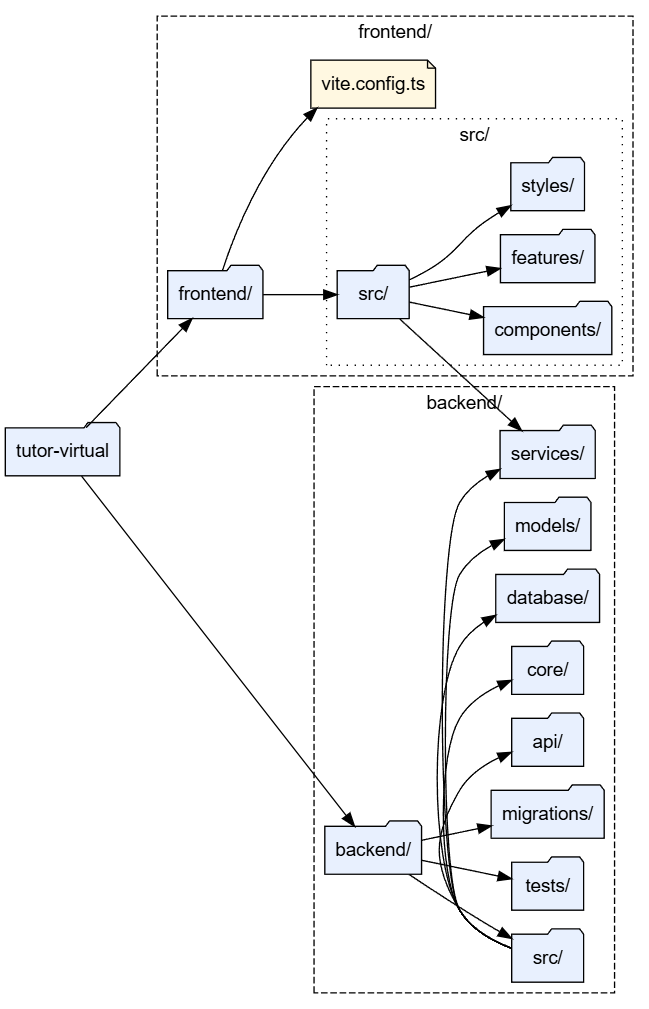
\includegraphics[width=0.8\linewidth]{Ilustraciones/folder_layers.png}
  \caption{Mapa conceptual de dependencias entre las principales capas y directorios del proyecto, ilustrando una arquitectura por niveles o \emph{feature-slices}.}
  \label{fig:desarrollo_folder-layers}
\end{figure}

%--------------------------------------------------------------------
\section{Iteración 1: Diseño e Implementación de la Base de Datos}
\label{sec:desarrollo_iter1_db}

Esta primera iteración de desarrollo se centró en establecer una \textbf{base de datos sólida y bien estructurada}. Las tareas principales incluyeron: (1) el modelado entidad-relación (E-R) basado en los requisitos iniciales; (2) la definición de una estrategia de migraciones de esquema utilizando Alembic; (3) el diseño del sistema de conexión a la base de datos PostgreSQL desde la aplicación FastAPI; y (4) la implementación de pruebas iniciales de consistencia del modelo.

%--------------------------------------------------------------------
\subsection{Modelado Entidad-Relación (E-R)}
\label{ssec:desarrollo_iter1_er}

El proceso de modelado E-R se llevó a cabo de la siguiente manera:
\begin{enumerate}[leftmargin=*]
  \item \textbf{Elicitación inicial de entidades:} A partir de los requisitos funcionales definidos en la Sección~\ref{ssec:desarrollo_reqs}, se identificaron las entidades núcleo del sistema: \texttt{Usuario (User)}, \texttt{Curso (Course)}, \texttt{Asignatura (Subject)}, y \texttt{Tema (Theme)}. Posteriormente se añadirían \texttt{Ejercicio (Exercise)} y \texttt{RespuestaUsuario (UserResponse)}.
  \item \textbf{Prototipado rápido con DBML:} Se utilizó la sintaxis DBML (\textit{Database Markup Language}) y herramientas online como \texttt{dbdiagram.io} para iterar rápidamente sobre el diseño del esquema, definir relaciones (incluyendo cardinalidades como uno-a-muchos y muchos-a-muchos) y tipos de datos.
  \item \textbf{Uso de tablas de asociación explícitas:} Para las relaciones muchos-a-muchos (ej. entre usuarios y cursos), se optó por el patrón de \emph{association table} (tabla de unión). Estas tablas intermedias, además de resolver la relación N:M, incluyen restricciones de unicidad (\texttt{UniqueConstraint}) para evitar registros duplicados y ofrecen la flexibilidad de añadir atributos adicionales a la relación en el futuro (p.ej., fecha de inscripción, rol específico en el curso, progreso).
\end{enumerate}

El diagrama E-R resultante de este proceso se muestra en la Figura~\ref{fig:er-diagram} (presentada previamente en el Capítulo~\ref{chap:aportaciones}, Sección~\ref{ssec:datamodel_aportaciones}).

%--------------------------------------------------------------------
\subsection{Estrategia y Plan de Migración con Alembic}
\label{ssec:desarrollo_iter1_migracion}

Para gestionar los cambios en el esquema de la base de datos de forma evolutiva y controlada, se implementó la siguiente estrategia con Alembic:
\begin{enumerate}[leftmargin=*]
  \item \textbf{Inicialización del entorno de Alembic:} Se ejecutó el comando \texttt{alembic init migrations} en el directorio raíz del backend (\texttt{tutor-backend/}). Esto generó la estructura de directorios necesaria para Alembic, incluyendo el archivo de configuración \texttt{alembic.ini} y el directorio\\ \texttt{migrations/versions/} donde se almacenan los scripts de migración. Se estableció una convención de nombres para los scripts de migración: \texttt{<timestamp>\_<breve\_descripcion\_del\_cambio>.py}.
  \item \textbf{Generación automática de revisiones:} Tras cada cambio en los modelos SQLAlchemy (definidos en \texttt{src/models/}), se utilizó el comando \texttt{alembic revision --autogenerate -m "descripcion del cambio"} para que Alembic comparara el estado actual de los modelos con el esquema de la base de datos (o el último estado conocido por Alembic) y generara automáticamente un nuevo script de migración con las operaciones DDL (Data Definition Language) necesarias (ej. \texttt{CREATE TABLE}, \texttt{ADD COLUMN}).
  \item \textbf{Revisión manual de scripts generados:} Antes de aplicar cualquier migración, los scripts generados fueron revisados manualmente. Esta revisión asegura la correcta definición de claves compuestas, restricciones (\emph{constraints}), índices, operaciones en cascada (\emph{cascades} para \texttt{ON DELETE} u \texttt{ON UPDATE}), y para añadir cualquier lógica de migración de datos que Alembic no pueda inferir automáticamente. Una vez revisado, el script se aplicaba a la base de datos con \texttt{alembic upgrade head}.
\end{enumerate}

%--------------------------------------------------------------------
\subsection{Diseño de la Conexión a la Base de Datos desde FastAPI}
\label{ssec:desarrollo_iter1_conexion}

La conexión y gestión de sesiones de base de datos desde la aplicación FastAPI se centralizó en el módulo \texttt{src/database/session.py}, cuyo contenido se muestra parcialmente en el Listado~\ref{lst:desarrollo_db-session}. Este diseño sigue el patrón de “\emph{session-per-request}” para APIs REST con SQLAlchemy:

\begin{itemize}[leftmargin=*]
  \item \textbf{Motor de base de datos síncrono (\texttt{create\_engine}):} Aunque FastAPI es asíncrono, para las operaciones de base de datos con SQLAlchemy se utilizó el motor síncrono. Las operaciones de BD suelen ser limitadas por E/S (\textit{I/O-bound}) y relativamente breves. SQLAlchemy gestiona un \emph{pool} de conexiones que ayuda a amortiguar la latencia de establecimiento de nuevas conexiones.
  \item \textbf{Factoría de Sesiones (\texttt{SessionLocal}):} Se define una factoría de sesiones utilizando \texttt{sessionmaker}. Es importante destacar la configuración \texttt{expire\_on\_commit=False}, que evita que SQLAlchemy invalide automáticamente todos los atributos de una instancia de modelo después de un \texttt{commit()}, lo cual previene la necesidad de realizar una segunda consulta SELECT si se accede a esos atributos post-commit dentro de la misma sesión.
  \item \textbf{Dependencia de FastAPI para la gestión de sesiones (\texttt{get\_db}):} Se creó una dependencia de FastAPI (\texttt{def get\_db() -> Generator[Session, None, None]: ...}) que se inyecta en las rutas de la API. Esta función maneja el ciclo de vida de una sesión de SQLAlchemy:
        \begin{enumerate}
            \item Abre una nueva sesión de forma \emph{lazy} (solo cuando se necesita) al inicio de una petición.
            \item Proporciona (\texttt{yield}) la sesión al endpoint de la API.
            \item Al finalizar la petición, intenta hacer \texttt{commit()} de la transacción si no hubo errores.
            \item En caso de cualquier excepción durante el procesamiento de la petición, realiza un \texttt{rollback()} para deshacer los cambios de la transacción actual.
            \item Finalmente, cierra la sesión (\texttt{db.close()}) para devolver la conexión al pool.
        \end{enumerate}
  \item \textbf{Gestión de variables de entorno para la conexión:} La URL de conexión a la base de datos (\texttt{DATABASE\_URL}) y otros parámetros sensibles se gestionan a través de variables de entorno, leídas por \texttt{src/core/config.py}.
\end{itemize}

\clearpage
\begin{lstlisting}[language=python,
                   caption={Gestión de la sesión de SQLAlchemy en \texttt{src/database/session.py} (extracto relevante).},
                   label={lst:desarrollo_db-session}, % Label actualizada
                   basicstyle=\fontsize{8}{9.5}\ttfamily]
"""Módulo para la gestión de la sesión de SQLAlchemy en la aplicación FastAPI."""

from typing import Generator
from sqlalchemy import create_engine, Engine
from sqlalchemy.orm import sessionmaker, Session

from src.core.config import get_app_settings, AppSettings

_SETTINGS: AppSettings = get_app_settings()

_DB_ENGINE: Engine | None = None

def get_engine() -> Engine:
    """
    Retorna una instancia singleton del motor de SQLAlchemy.
    Crea el motor si no existe, utilizando la configuración de la aplicación.
    """
    global _DB_ENGINE
    if _DB_ENGINE is None:
        _DB_ENGINE = create_engine(
            str(_SETTINGS.DATABASE_URL),
            pool_size=_SETTINGS.DB_POOL_SIZE,
            max_overflow=_SETTINGS.DB_MAX_OVERFLOW,
            echo=_SETTINGS.DB_ECHO_SQL,
            future=True
        )
    return _DB_ENGINE

SessionLocal = sessionmaker(
    bind=get_engine(),
    autocommit=False,
    autoflush=False,
    expire_on_commit=False
)

def get_db() -> Generator[Session, None, None]:
    """
    Dependencia de FastAPI para obtener una sesión de base de datos por petición.
    Maneja el ciclo de vida de la sesión: la crea, la proporciona,
    hace commit o rollback, y finalmente la cierra.
    """
    db: Session = SessionLocal()
    try:
        yield db
        db.commit()endpoint
    except Exception:
        db.rollback()
        raise
    finally:
        db.close()
\end{lstlisting}

Este enfoque asegura que cada petición a la API opere dentro de su propia transacción de base de datos, manteniendo la consistencia y el aislamiento. Las migraciones, generadas con \texttt{alembic revision --autogenerate -m "mensaje"}, se aplican de forma controlada, y su validez se comprueba en el pipeline de CI/CD con \texttt{alembic upgrade head} asegurando la integridad del esquema antes de cualquier despliegue.

%--------------------------------------------------------------------
\section{Iteración 2: Desarrollo del Backend RESTful con FastAPI}
\label{sec:desarrollo_iter2_backend}

Una vez establecida la base de datos y la estrategia de migraciones, la segunda iteración se enfocó en construir la API RESTful utilizando FastAPI. El objetivo era exponer la lógica de negocio y los datos del sistema de manera segura y eficiente.

%--------------------------------------------------------------------
\subsection{Configuración del Proyecto FastAPI y Estructura}
\label{ssec:desarrollo_iter2_config}

La configuración inicial del proyecto FastAPI incluyó:
\begin{itemize}[leftmargin=*]
  \item \textbf{Estructura de directorios:} Se siguió la estructura detallada en la Sección~\ref{sssec:desarrollo_arch_backend}, promoviendo la separación de responsabilidades (API, core, base de datos, modelos, servicios).
  \item \textbf{Configuración centralizada (\texttt{src/core/config.py}):} Se utilizó Pydantic Settings para cargar la configuración desde variables de entorno. Esto permite gestionar de forma centralizada parámetros como la URL de la base de datos, secretos de JWT, configuraciones de CORS, etc. El Listado~\ref{lst:desarrollo_settings} muestra un extracto de esta configuración.
  \item \textbf{Middlewares esenciales:} Se configuraron middlewares para:
        \begin{itemize}
            \item \textbf{CORS (\emph{Cross-Origin Resource Sharing}):} Para permitir peticiones desde el frontend ( \texttt{http://localhost:5173} durante el desarrollo).
            \item \textbf{Manejo global de excepciones:} Para capturar errores no controlados y devolver respuestas HTTP estandarizadas.
        \end{itemize}
\end{itemize}

\clearpage
\begin{lstlisting}[language=python,
                   caption={Extracto del objeto de configuración global (\texttt{src/core/config.py}) utilizando Pydantic Settings.},
                   label={lst:desarrollo_settings}, % Label actualizada
                   basicstyle=\fontsize{8}{9.5}\ttfamily]
from pydantic import Field, PostgresDsn, HttpUrl
from pydantic_settings import BaseSettings, SettingsConfigDict
from typing import List, Optional

class AppSettings(BaseSettings):
    model_config = SettingsConfigDict(
        env_file=".env",
        env_file_encoding="utf-8",
        case_sensitive=False,
        extra='ignore'  # Ignorar variables extra en .env
    )

    API_TITLE: str = "Tutor Virtual API"
    API_VERSION: str = "0.1.0"
    API_V1_STR: str = "/api/v1"
    DEBUG_MODE: bool = Field(False, env="DEBUG_MODE")
    CORS_ORIGINS: List[HttpUrl] = Field(default_factory=list, env="CORS_ORIGINS")
    DATABASE_URL: PostgresDsn = Field(..., env="DATABASE_URL") # URL de conexión a PostgreSQL (obligatoria)
    DB_POOL_SIZE: int = Field(10, env="DB_POOL_SIZE")
    DB_MAX_OVERFLOW: int = Field(20, env="DB_MAX_OVERFLOW")
    DB_ECHO_SQL: bool = Field(False, env="DB_ECHO_SQL")
    
    JWT_SECRET_KEY: str = Field(..., env="JWT_SECRET_KEY", min_length=32)
    JWT_ALGORITHM: str = "HS256"
    JWT_ACCESS_TOKEN_EXPIRE_MINUTES: int = Field(30, env="JWT_ACCESS_TOKEN_EXPIRE_MINUTES")
    JWT_REFRESH_TOKEN_EXPIRE_DAYS: int = Field(7, env="JWT_REFRESH_TOKEN_EXPIRE_DAYS")
    PASSWORD_HASHER_ROUNDS: int = Field(12, env="PASSWORD_HASHER_ROUNDS")

    GOOGLE_CLIENT_ID: Optional[str] = Field(None, env="GOOGLE_CLIENT_ID")
    GOOGLE_CLIENT_SECRET: Optional[str] = Field(None, env="GOOGLE_CLIENT_SECRET")
    GOOGLE_REDIRECT_URI: Optional[HttpUrl] = Field(None, env="GOOGLE_REDIRECT_URI")

    OLLAMA_API_BASE_URL: HttpUrl = Field("http://localhost:11434", env="OLLAMA_API_BASE_URL")
    AI_REQUEST_TIMEOUT_SECONDS: int = Field(60, env="AI_REQUEST_TIMEOUT_SECONDS") # Timeout para peticiones a la IA

    ENVIRONMENT: str = Field("dev", env="ENVIRONMENT")
    AUTO_CREATE_DATABASE_TABLES_ON_STARTUP: bool = Field(False, env="AUTO_CREATE_DATABASE_TABLES_ON_STARTUP")
    RUN_MIGRATIONS_ON_STARTUP: bool = Field(False, env="RUN_MIGRATIONS_ON_STARTUP")

_app_settings_instance: Optional[AppSettings] = None

def get_app_settings() -> AppSettings:
    global _app_settings_instance
    if _app_settings_instance is None:
        _app_settings_instance = AppSettings()
    return _app_settings_instance
\end{lstlisting}

%--------------------------------------------------------------------
\subsection{Desarrollo del Módulo de Autenticación y Gestión de Usuarios}
\label{ssec:desarrollo_iter2_auth}

Se implementó un sistema de autenticación robusto basado en JWT (JSON Web Tokens) y se ofreció la opción de registro/login con Google OAuth 2.0.

\paragraph{Flujo de Autenticación con JWT y OAuth 2.0.}
El sistema de autenticación sigue estos flujos principales:
\begin{enumerate}[label=\alph*),leftmargin=*]
  \item \textbf{Registro de nuevos usuarios (\texttt{POST /api/auth/register}):} Permite el alta de usuarios mediante un nombre de usuario, correo electrónico y contraseña. El sistema verifica la unicidad del nombre de usuario y del correo electrónico. La contraseña se almacena de forma segura utilizando hashing con \texttt{bcrypt} (específicamente, \texttt{bcrypt\_sha256} a través de una biblioteca como \texttt{passlib}). El controlador para esta ruta se muestra en el Listado~\ref{lst:desarrollo_register_controller}.

  \item \textbf{Inicio de sesión (\texttt{POST /api/auth/login}):} Los usuarios se autentican con su correo electrónico y contraseña. Si las credenciales son válidas (verificando la contraseña hasheada), el servidor genera y devuelve un par de tokens JWT:
        \begin{itemize}
            \item \textbf{Token de Acceso (\emph{Access Token}):} De corta duración. Se utiliza para autorizar el acceso a rutas protegidas de la API.
            \item \textbf{Token de Refresco (\emph{Refresh Token}):} De larga duración. Se utiliza para obtener nuevos tokens de acceso sin que el usuario tenga que volver a introducir sus credenciales. Este token se almacena de forma segura en la base de datos y se invalida tras su uso (rotación de tokens de refresco) o al cerrar sesión.
        \end{itemize}

  \item \textbf{Refresco de tokens (\texttt{POST /api/auth/refresh}):} Cuando el token de acceso expira, el cliente puede solicitar un nuevo par de tokens enviando el token de refresco vigente. El servidor valida el token de refresco contra la base de datos, verifica su caducidad y, si es válido, emite un nuevo token de acceso y un nuevo token de refresco.

  \item \textbf{Autenticación con Google (\texttt{POST /api/auth/google}):} Se implementó el flujo de OAuth 2.0 para "aplicaciones web del lado del servidor". De forma simplificada:
        \begin{enumerate}
            \item El frontend redirige al usuario a la página de consentimiento de Google.
            \item Tras el consentimiento, Google redirige de nuevo al frontend con un código de autorización (\emph{authorization code}).
            \item El frontend envía este código de autorización al backend (\texttt{/api/auth/google}).
            \item El backend intercambia este código con Google por un \emph{ID token} y un \emph{access token} de Google.
            \item El backend verifica la firma y la información del \emph{ID token} de Google (utilizando la biblioteca \texttt{google-auth}).
            \item Si la verificación es exitosa, el backend crea una cuenta de usuario local si no existe (o recupera la existente si el correo ya está registrado) y emite sus propios tokens JWT (acceso y refresco) para el usuario, que se devuelven al frontend.
        \end{enumerate}
\end{enumerate}

\paragraph{Protección de Rutas con Dependencias de Seguridad.}
Las rutas de la API que requieren autenticación se protegen utilizando dependencias de FastAPI. Se creó una dependencia \texttt{jwt\_required} que:
\begin{enumerate}
    \item Obtiene el token JWT del encabezado \texttt{Authorization: Bearer <token>}.
    \item Valida la firma del token utilizando la clave secreta (\texttt{JWT\_SECRET\_KEY}) y el algoritmo especificado (\texttt{JWT\_ALGORITHM}, ej. HS256).
    \item Verifica la fecha de expiración del token.
    \item Si todas las validaciones son correctas, extrae la información del usuario (\emph{payload}, ej. \texttt{user\_id}) y la hace disponible para el endpoint. En caso contrario, lanza una excepción \texttt{HTTPException} (ej. \texttt{401 Unauthorized}).
\end{enumerate}
Para rutas que requieren privilegios de administrador, se creó una dependencia adicional \texttt{admin\_required} que primero invoca a \texttt{jwt\_required} y luego verifica un \emph{claim} de administrador en el \emph{payload} del token (ej. \texttt{is\_admin: true}). El Listado~\ref{lst:desarrollo_jwt-guards} muestra una implementación simplificada de estas dependencias.

\paragraph{Limitación de Tasa de Peticiones (\emph{Rate Limiting}).}
Para proteger la API contra abusos y ataques de fuerza bruta, se puede integrar una biblioteca como \texttt{slowapi}. Esta permite definir límites de peticiones (ej. 20 peticiones por minuto por IP) para ciertos endpoints, especialmente los de autenticación. Si se excede el límite, la API devuelve una respuesta \texttt{HTTP 429 Too Many Requests}.

\clearpage
\begin{lstlisting}[language=python,
                   caption={Controlador para el registro de usuarios (\texttt{src/api/routes/auth.py} - extracto).},
                   label={lst:desarrollo_register_controller}, % Label actualizada
                   basicstyle=\fontsize{8}{9.5}\ttfamily]
from fastapi import APIRouter, Depends, HTTPException, status
from sqlalchemy.orm import Session
from sqlalchemy.exc import IntegrityError

from src.api.dependencies.database import get_db
from src.api.schemas.auth import UserCreateIn, UserPublicOut
from src.models.user import User as UserModel
from src.core.security import hash_password
from src.services.user_service import get_user_by_email, get_user_by_username

router = APIRouter(prefix="/auth", tags=["Authentication"])

@router.post(
    "/register",
    response_model=UserPublicOut,
    status_code=status.HTTP_201_CREATED,
    summary="Register a new user",
    description="Creates a new user account if the username and email are not already taken."
)
def register_user(
    user_in: UserCreateIn,
    db: Session = Depends(get_db)
) -> UserPublicOut:
    existing_user_by_username = get_user_by_username(db, username=user_in.username)
    if existing_user_by_username:
        raise HTTPException(
            status_code=status.HTTP_409_CONFLICT,
            detail="Username already registered."
        )

    existing_user_by_email = get_user_by_email(db, email=user_in.email)
    if existing_user_by_email:
        raise HTTPException(
            status_code=status.HTTP_409_CONFLICT,
            detail="Email already registered."
        )

    hashed_password = hash_password(user_in.password)
    new_user = UserModel(
        username=user_in.username,
        email=user_in.email,
        hashed_password=hashed_password,
    )
    
    db.add(new_user)
    try:
        db.commit()
        db.refresh(new_user)
    except IntegrityError:
        db.rollback()
        raise HTTPException(
            status_code=status.HTTP_500_INTERNAL_SERVER_ERROR,
            detail="Could not create user due to a database conflict."
        ) from None

    return UserPublicOut.model_validate(new_user)
\end{lstlisting}

\clearpage

\begin{lstlisting}[language=python,
                   caption={Dependencias de seguridad \texttt{jwt\_required} y \texttt{admin\_required} (simplificadas - \texttt{src/api/dependencies/auth.py}).},
                   label={lst:desarrollo_jwt-guards}, % Label actualizada
                   basicstyle=\fontsize{8}{9.5}\ttfamily]
from fastapi import Depends, HTTPException, status
from fastapi.security import HTTPBearer, HTTPAuthorizationCredentials
from jose import JWTError, jwt
from pydantic import BaseModel, ValidationError

from src.core.config import get_app_settings, AppSettings
from src.api.schemas.auth import TokenPayload
from src.services.user_service import get_user_by_id
from sqlalchemy.orm import Session
from src.api.dependencies.database import get_db

_SETTINGS: AppSettings = get_app_settings()
http_bearer_scheme = HTTPBearer(description="JWT Access Token")

class AuthenticatedUser(BaseModel):
    id: int
    username: str
    email: str
    is_admin: bool

def get_current_user_payload(
    token: HTTPAuthorizationCredentials = Depends(http_bearer_scheme)
) -> TokenPayload:
    """Decodifica y valida el token JWT, retorna el payload."""
    if token is None:
        raise HTTPException(
            status_code=status.HTTP_401_UNAUTHORIZED,
            detail="Not authenticated: Missing token.",
            headers={"WWW-Authenticate": "Bearer"},
        )
    try:
        payload_dict = jwt.decode(
            token.credentials,
            _SETTINGS.JWT_SECRET_KEY,
            algorithms=[_SETTINGS.JWT_ALGORITHM]
        )
        token_payload = TokenPayload(**payload_dict)
    except (JWTError, ValidationError) as e:
        raise HTTPException(
            status_code=status.HTTP_401_UNAUTHORIZED,
            detail="Could not validate credentials: Invalid or expired token.",
            headers={"WWW-Authenticate": "Bearer"},
        )
    return token_payload

def jwt_required(
    payload: TokenPayload = Depends(get_current_user_payload),
    db: Session = Depends(get_db)
) -> AuthenticatedUser:
    """
    Dependencia para requerir un JWT válido.
    Obtiene el usuario de la BD a partir del ID en el payload del token.
    """
    if payload.user_id is None:
        raise HTTPException(status_code=status.HTTP_400_BAD_REQUEST, detail="Invalid token payload: user_id missing.")

    user = get_user_by_id(db, user_id=payload.user_id)
    if user is None:
        raise HTTPException(status_code=status.HTTP_404_NOT_FOUND, detail="User not found.")

    return AuthenticatedUser(
        id=user.id,
        username=user.username,
        email=user.email,
        is_admin=user.is_admin
    )

def admin_required(current_user: AuthenticatedUser = Depends(jwt_required)) -> AuthenticatedUser:
    """
    Dependencia para requerir que el usuario autenticado sea administrador.
    Reutiliza jwt_required para asegurar la autenticación primero.
    """
    if not current_user.is_admin:
        raise HTTPException(
            status_code=status.HTTP_403_FORBIDDEN,
            detail="Operation not permitted: Administrator privileges required."
        )
    return current_user
\end{lstlisting}

%--------------------------------------------------------------------
\subsection{Integración con el Motor de Inteligencia Artificial (IA)}
\label{ssec:desarrollo_iter2_ai}

El backend actúa como un intermediario (\emph{proxy}) entre el frontend y el motor de IA local (desplegado en Docker con OpenWebUI y llama.cpp). Se implementó una ruta que gestiona esta comunicación:

\begin{itemize}[leftmargin=*]
  \item \textbf{Cliente HTTP asíncrono (\texttt{httpx}):} Para realizar peticiones al servicio de IA local (escuchando en \texttt{http://localhost:3000}, configurable vía \texttt{OLLAMA\_API\_BASE\_URL}), se utilizó la biblioteca \texttt{httpx.AsyncClient}. Esto permite que el backend maneje las peticiones a la IA de forma no bloqueante, liberando los \emph{workers} de FastAPI para atender otras peticiones mientras se espera la respuesta de la IA. Se configuró un \emph{timeout} adecuado para estas peticiones.
  \item \textbf{Gestión de la fase de \emph{warm-up} del LLM:} Es importante notar que la primera petición al motor de IA después de su inicio puede tardar significativamente más (ej. 7-10 segundos) debido a la carga del modelo LLM en memoria. Las peticiones siguientes son mucho más rápidas (ej. \( \le \SI{1}{s} \)). El backend no gestiona explícitamente este \emph{warm-up}; simplemente espera la respuesta dentro del timeout configurado.
  \item \textbf{Formato del \emph{payload} de entrada a la IA:} La petición que el backend envía al motor de IA se construye en el formato esperado por la API de Ollama. Un ejemplo de este formato (JSON) se muestra en el Listado~\ref{lst:desarrollo_ollama-req-payload}. Este \emph{payload} incluye el nombre del modelo a utilizar, el formato de respuesta esperado, y los mensajes de la conversación.
  \item \textbf{Validación y normalización de la respuesta de la IA:} La respuesta JSON recibida del motor de IA se valida utilizando un schema Pydantic en el backend (ej. \texttt{AIExerciseOut}, mostrado en el Listado~\ref{lst:desarrollo_ai-schema_response}) antes de ser reenviada al frontend. Esto asegura que la respuesta tenga la estructura y los campos esperados (ej. \texttt{id}, \texttt{tema}, \texttt{enunciado}, \texttt{dificultad}, \texttt{tipo}, \texttt{explicacion}), y permite manejar errores si la IA devuelve una respuesta malformada.
\end{itemize}

\begin{lstlisting}[language=json,
                   caption={Ejemplo de payload de petición al motor de IA (formato Ollama).},
                   label={lst:desarrollo_ollama-req-payload}, % Label actualizada
                   basicstyle=\fontsize{8}{9.5}\ttfamily]
{
  "model": "profesor_generador_ejercicios",
  "format": "json", // Solicita que la respuesta del LLM sea un JSON válido
  "stream": false, // Para este caso, no se necesita streaming
  "system": "Eres un tutor virtual experto en generar ejercicios educativos concisos y claros. El ejercicio debe ser autoevaluable y tener una respuesta única y bien definida. Proporciona también una explicación breve y clara de cómo resolverlo.",
  "prompt": "Genera un ejercicio de nivel {{difficulty}} sobre el tema \"{{theme_title}}\". El ejercicio debe ser de tipo {{exercise_type}}.",
  "options": { // Opciones específicas del modelo LLM
    "temperature": 0.7,
    "num_predict": 256 // Limita el número máximo de tokens en la respuesta
  }
}
\end{lstlisting}

\begin{lstlisting}[language=python,
                   caption={Schema Pydantic (\texttt{AIExerciseOut}) para validar la respuesta JSON del motor de IA.},
                   label={lst:desarrollo_ai-schema_response}, % Label actualizada
                   basicstyle=\fontsize{8}{9.5}\ttfamily]
from pydantic import BaseModel, Field, validator
from typing import Optional, Literal

class AIExerciseOut(BaseModel):
    
    tema: str = Field(..., description="El tema principal del ejercicio.")
    enunciado: str = Field(..., description="El enunciado completo del ejercicio.")
    dificultad: Literal["fácil", "intermedio", "difícil"] = Field(..., description="Nivel de dificultad del ejercicio.")
    tipo: str = Field(..., description="Tipo de ejercicio (ej. opción múltiple, respuesta corta).")
    explicacion: Optional[str] = Field(None, description="Explicación detallada de la solución.")

    @validator("enunciado")
    def enunciado_must_not_be_empty(cls, value):
        if not value.strip():
            raise ValueError("El enunciado no puede estar vacío.")
        return value
\end{lstlisting}

%--------------------------------------------------------------------
\subsection{Implementación de Pruebas Unitarias y de Integración}
\label{ssec:desarrollo_iter2_tests}

Se puso un fuerte énfasis en las pruebas automatizadas para asegurar la calidad y fiabilidad del backend.

\paragraph{a) Configuración Unificada de Pruebas con \texttt{conftest.py}.}
Se utilizó un archivo \texttt{conftest.py} en el directorio de pruebas para definir \emph{fixtures} de Pytest reutilizables y configurar el entorno de pruebas. Puntos clave de esta configuración (ver extracto en Listado~\ref{lst:desarrollo_conftest}):
\begin{enumerate}[leftmargin=*]
  \item \textbf{Mocking de dependencias externas:} Para evitar la necesidad de instalar el cliente nativo de PostgreSQL en el entorno de CI o en máquinas de desarrolladores que solo ejecutan pruebas unitarias, se puede utilizar una técnica de \emph{mocking} a nivel de módulo.
  \item \textbf{Base de datos SQLite en memoria para pruebas:} Para la mayoría de las pruebas, se utilizó una base de datos SQLite en memoria \\ (\texttt{sqlite:///:memory:}) en lugar de una instancia real de PostgreSQL. Esto acelera la ejecución de las pruebas. Se configuró el motor SQLAlchemy con \texttt{StaticPool} para asegurar que cada prueba (o sesión de pruebas) utilice la misma conexión en memoria. Alembic se utilizó para aplicar el esquema completo de la base de datos a esta instancia SQLite una única vez por sesión de pruebas.
  \item \textbf{Cliente de pruebas de FastAPI configurado:} Se creó una \emph{fixture} de Pytest que proporciona una instancia de \texttt{TestClient} preconfigurada. Esta configuración incluye \emph{overrides} de dependencias de FastAPI:
        \begin{itemize}
            \item La dependencia \texttt{get\_db} se sobrescribe para que utilice la sesión de la base de datos SQLite en memoria.
            \item Las dependencias de seguridad como \texttt{jwt\_required} y \texttt{admin\_required} se sobrescriben con \emph{stubs} (funciones falsas) que devuelven un usuario autenticado y/o administrador simulado (\texttt{\{"user\_id": 1, "is\_admin": True\}}). Esto permite probar los endpoints protegidos sin necesidad de pasar por todo el flujo de autenticación en cada prueba.
        \end{itemize}
  \item \textbf{Limpieza automática del entorno entre pruebas (\emph{Test Hygiene}):}
        \begin{itemize}
           \item Reseteo de la configuración de \emph{logging} para evitar interferencias entre pruebas.
           \item Truncado (o borrado y recreación) de todas las tablas de la base de datos SQLite entre cada prueba (o al final de cada prueba) para asegurar el aislamiento de los tests.
           \item Vaciado de cachés internas, como la caché de la función \texttt{get\_app\_settings}, para asegurar que cada prueba comience con una configuración limpia.
        \end{itemize}
\end{enumerate}

\begin{lstlisting}[language=python,
                   caption={Extracto abreviado y conceptual de \texttt{conftest.py} para configurar el entorno de pruebas de FastAPI.},
                   label={lst:desarrollo_conftest}, % Label actualizada
                   basicstyle=\fontsize{8}{9.5}\ttfamily]
import pytest
from typing import Generator
from fastapi.testclient import TestClient
from sqlalchemy import create_engine, StaticPool
from sqlalchemy.orm import Session, sessionmaker

from src.main import app as fastapi_app tiene create_app() o la instancia app
from src.core.config import get_app_settings, AppSettings
from src.database.session import get_db
from src.models.base import Base
from src.api.dependencies.auth import jwt_required, admin_required


@pytest.fixture(scope="session")
def db_engine():
    """Crea un motor SQLAlchemy para una base de datos SQLite en memoria para las pruebas."""
    engine = create_engine(
        "sqlite:///:memory:",
        connect_args={"check_same_thread": False},
        poolclass=StaticPool,
        future=True
    )
    Base.metadata.create_all(bind=engine)
    yield engine

@pytest.fixture(scope="function")
def db_session(db_engine) -> Generator[Session, None, None]:
    """Crea una nueva sesión de base de datos para cada prueba, con rollback al final."""
    connection = db_engine.connect()
    transaction = connection.begin()
    
    TestingSessionLocal = sessionmaker(autocommit=False, autoflush=False, bind=connection, future=True)
    session = TestingSessionLocal()
    
    yield session
    
    session.close()
    transaction.rollback()
    connection.close()

@pytest.fixture(scope="function")
def test_client(db_session: Session) -> Generator[TestClient, None, None]:
    """
    Crea una instancia de TestClient de FastAPI con dependencias sobrescritas
    para usar la sesión de BD de prueba y mockear la autenticación.
    """
    
    def override_jwt_required():
        return {"user_id": 1, "username": "testuser", "email": "test@example.com", "is_admin": False}

    def override_admin_required():
        return {"user_id": 1, "username": "testadmin", "email": "admin@example.com", "is_admin": True}

    fastapi_app.dependency_overrides[get_db] = lambda: db_session
    fastapi_app.dependency_overrides[jwt_required] = override_jwt_required
    fastapi_app.dependency_overrides[admin_required] = override_admin_required
    
    with TestClient(fastapi_app) as client:
        yield client

    fastapi_app.dependency_overrides.clear()
\end{lstlisting}

\paragraph{b) Cobertura de Pruebas Unitarias.}
Se desarrollaron pruebas unitarias para verificar la lógica de componentes individuales en aislamiento:
\begin{itemize}[leftmargin=*]
  \item \textbf{Autenticación y Autorización:} Se escribieron pruebas para los decoradores/dependencias de seguridad (\texttt{jwt\_required}, \texttt{admin\_required}), cubriendo casos como token ausente, token inválido/expirado, usuario no administrador intentando acceder a rutas de administrador, y acceso correcto. El Listado~\ref{lst:desarrollo_auth-tests_unit} muestra un ejemplo de estas pruebas.
  \item \textbf{Schemas Pydantic:} Se probaron los modelos Pydantic (ej. para \texttt{UserCreateIn}, \texttt{AnswerIn/Out}) para asegurar que la validación de tipos, restricciones de longitud, formatos (ej. email), y campos obligatorios funcionaran como se esperaba.
  \item \textbf{Servicios y Lógica de Negocio:} Se probaron funciones críticas en los módulos de servicios (ej. \texttt{user\_service.py}), mockeando las interacciones con la base de datos cuando era necesario para aislar la lógica de negocio.
  \item \textbf{Utilidades (ej. Cliente de IA):} Se probó la lógica del cliente HTTP para interactuar con el motor de IA (\texttt{generate\_with\_ollama}), incluyendo el manejo de \emph{timeouts}, reintentos, y la correcta formación de cabeceras.
\end{itemize}

\begin{lstlisting}[language=python,
                   caption={Extracto de pruebas unitarias para dependencias de autenticación (\texttt{tests/unit/api/dependencies/test\_auth\_dependency.py}).},
                   label={lst:desarrollo_auth-tests_unit}, % Label actualizada
                   basicstyle=\fontsize{8}{9.5}\ttfamily]
import pytest
from fastapi import HTTPException, status
from jose import jwt

from src.api.dependencies.auth import get_current_user_payload, jwt_required, admin_required, AuthenticatedUser, TokenPayload
from src.core.config import get_app_settings

_SETTINGS = get_app_settings()

def test_get_current_user_payload_valid_token():
    test_payload_data = {"user_id": 123, "username": "testuser", "exp": 9999999999}
    token = jwt.encode(test_payload_data, _SETTINGS.JWT_SECRET_KEY, algorithm=_SETTINGS.JWT_ALGORITHM)
    
    class MockHTTPAuthCreds:
        scheme = "Bearer"
        credentials = token
    
    payload = get_current_user_payload(token=MockHTTPAuthCreds())
    assert payload.user_id == test_payload_data["user_id"]
    assert payload.username == test_payload_data["username"]

def test_get_current_user_payload_missing_token():
    with pytest.raises(HTTPException) as exc_info:
        get_current_user_payload(token=None)
    assert exc_info.value.status_code == status.HTTP_401_UNAUTHORIZED
    assert "Missing token" in exc_info.value.detail

def test_get_current_user_payload_invalid_token_format():
    class MockHTTPAuthCreds:
        scheme = "Bearer"
        credentials = "this.is.not.a.valid.jwt"
        
    with pytest.raises(HTTPException) as exc_info:
        get_current_user_payload(token=MockHTTPAuthCreds())
    assert exc_info.value.status_code == status.HTTP_401_UNAUTHORIZED
    assert "Invalid or expired token" in exc_info.value.detail

def test_admin_required_is_admin():
    mock_admin_user = AuthenticatedUser(id=1, username="admin", email="admin@example.com", is_admin=True)
    result = admin_required(current_user=mock_admin_user)
    assert result == mock_admin_user

def test_admin_required_not_admin():
    mock_normal_user = AuthenticatedUser(id=2, username="user", email="user@example.com", is_admin=False)
    with pytest.raises(HTTPException) as exc_info:
        admin_required(current_user=mock_normal_user)
    assert exc_info.value.status_code == status.HTTP_403_FORBIDDEN
    assert "Administrator privileges required" in exc_info.value.detail
\end{lstlisting}

\paragraph{c) Cobertura de Pruebas de Integración.}
Las pruebas de integración se enfocaron en verificar el comportamiento de los endpoints de la API en conjunto con la lógica de negocio y (una versión mockeada o en memoria de) la base de datos:
\begin{itemize}
    \item Se probaron los flujos CRUD completos para las entidades principales (usuarios, cursos, asignaturas, temas).
    \item Se verificó el funcionamiento de la autenticación y autorización a nivel de endpoint.
    \item Se validaron los códigos de estado HTTP, los formatos de respuesta y el manejo de errores para diferentes escenarios de entrada.
\end{itemize}

Este enfoque de pruebas permitió la estabilidad y fiabilidad del backend.

%--------------------------------------------------------------------
\section{Iteración 3: Desarrollo del Frontend con React y Vite}
\label{sec:desarrollo_iter3_frontend}

Con el backend y la base de datos establecidos, el objetivo de la tercera iteración fue desarrollar una \textbf{interfaz de usuario (frontend) funcional y completa}. Esta interfaz debía consumir la API RESTful creada en la Iteración 2 y permitir tanto a estudiantes como a administradores interactuar con el sistema de manera intuitiva. Se puso énfasis en la creación de una experiencia de usuario (UX) fluida, responsiva y accesible.

%--------------------------------------------------------------------
\subsection{Desarrollo de las Principales Pantallas y Flujos de Usuario}
\label{ssec:desarrollo_iter3_pantallas}

Se desarrollaron varias pantallas clave, cada una con sus propios componentes y lógica de estado.

%------------------------------------------------
\subsubsection{Página de Aterrizaje (Landing Page - \texttt{/})}
\label{sssec:desarrollo_landing_page}

\begin{itemize}[leftmargin=*]
  \item \textbf{Propósito y Diseño:} La página de aterrizaje fue diseñada para ser la primera impresión de la marca \textbf{Tutor Virtual}. Su objetivo es comunicar claramente la propuesta de valor de la aplicación y guiar al usuario hacia la acción principal (registro o inicio de sesión). El diseño sigue el principio de marketing de las "3 H": \textit{Hook} (captar la atención), \textit{Hold} (mantener el interés explicando los beneficios) y \textit{Hand-off} (dirigir al siguiente paso, \texttt{/register}).

  \item \textbf{Accesibilidad (A11y):}
        \begin{itemize}
          \item Se aseguró una jerarquía de encabezados correcta (un solo \texttt{<h1>} por página, uso adecuado de \texttt{<h2>}, \texttt{<h3>}, etc.).
          \item Todos los elementos interactivos (botones, enlaces, controles de carrusel) se hicieron accesibles mediante teclado y se les proporcionaron etiquetas ARIA adecuadas (ej. \texttt{aria-label} para botones con solo iconos).
          \item Se verificó el contraste de color.
          \item Todos los botones utilizan el elemento semántico \texttt{<button>} o, si se construyen con \texttt{<div>} o \texttt{<a>}, se les asigna \texttt{role="button"} y \texttt{tabIndex=0}, además de manejar eventos de teclado (\texttt{onClick}, \texttt{onKeyDown} para Enter/Espacio).
        \end{itemize}

  \item \textbf{Rendimiento Web y SEO:}
        \begin{itemize}
          \item Carga diferida (\texttt{loading="lazy"}) para imágenes que no están en el \emph{viewport} inicial.
          \item Uso de \texttt{<link rel="preload">} o \texttt{<link rel="preconnect">} para fuentes web críticas o dominios de terceros importantes para acelerar la carga percibida y mejorar métricas como LCP (\textit{Largest Contentful Paint}).
          \item Optimización del \emph{bundle} de JavaScript mediante técnicas de \emph{code splitting} de Vite. React Router 6 puede ayudar con la precarga de \emph{chunks} de rutas (\texttt{prefetch="intent"}) al pasar el cursor sobre enlaces a páginas clave.
        \end{itemize}
\end{itemize}

%------------------------------------------------
\subsubsection{Autenticación (\texttt{/login}, \texttt{/register})}
\label{sssec:desarrollo_auth_pages}

\begin{itemize}[leftmargin=*]
  \item \textbf{Gestión de Formularios con React Hook Form y Zod:} Para los formularios de inicio de sesión y registro, se utilizó la biblioteca \texttt{react-hook-form} junto con \texttt{zod} para la validación de esquemas. Esta combinación ofrece:
        \begin{itemize}
            \item \textbf{Rendimiento:} React Hook Form minimiza los re-renderizados al delegar el estado a los propios inputs (utilizando referencias no controladas o \texttt{ref}), en lugar de un estado de React para cada campo.
            \item \textbf{Validación declarativa:} Zod permite definir esquemas de validación de forma clara y concisa (ej. \texttt{z.string().min(8)}, \texttt{z.string().email()}), que se integran fácilmente con React Hook Form a través de un \emph{resolver} (\texttt{@hookform/resolvers/zod}).
        \end{itemize}

  \item \textbf{Formulario de Inicio de Sesión (\texttt{LoginForm.tsx}):}
        \begin{itemize}
          \item Campos para \texttt{email} y \texttt{password}. Los mensajes de error de validación se muestran en línea, asociados a cada campo (ej. \texttt{errors.email?.message}).
          \item Utiliza un hook de mutación de React Query (ej. \texttt{useLoginMutation}) que realiza la petición \texttt{POST /api/auth/login} al backend.
          \item En caso de éxito, se invoca la función \texttt{login()} del contexto de autenticación (pasando los tokens de acceso y refresco) y se redirige al usuario al panel principal (\texttt{/dashboard}) utilizando \texttt{navigate('/dashboard', \{ replace: true \})} para evitar que la página de login quede en el historial del navegador.
          \item El botón de envío se deshabilita y muestra un indicador de carga (ej. "Iniciando sesión...") mientras la mutación está pendiente \\ (\texttt{mutation.isPending}).
        \end{itemize}

  \item \textbf{Formulario de Registro (\texttt{RegisterForm.tsx}):}
        \begin{itemize}
          \item Campos para \texttt{username}, \texttt{email}, \texttt{password} y \texttt{confirmPassword}. Se aplican estilos para asegurar un buen contraste y feedback visual en los inputs (ej. cambio de borde en \texttt{:focus}).
          \item Incluye una casilla de verificación (\emph{checkbox}) para aceptar los términos y condiciones, que debe estar marcada para habilitar el envío del formulario.
          \item Tras un registro exitoso (gestionado también con un hook de mutación de React Query), se redirige al usuario a la página de inicio de sesión (\texttt{/login}) con \texttt{replace: true}.
        \end{itemize}

  \item \textbf{Botón de Inicio de Sesión con Google (\texttt{MyGoogleButton.tsx}):}
        \begin{itemize}
          \item Utiliza la biblioteca \texttt{@react-oauth/google} para implementar el flujo de inicio de sesión con Google. Específicamente, el flujo ''auth-code'' (\texttt{useGoogleLogin(\{ flow: 'auth-code' \})}) es el recomendado para interactuar con un backend propio.
          \item Al obtener el código de autorización de Google, este se envía al endpoint del backend (\texttt{/api/auth/google}).
          \item El backend intercambia el código por tokens y, si tiene éxito, devuelve los tokens JWT propios de la aplicación.
          \item El frontend entonces llama a la función \texttt{login()} del contexto de autenticación y redirige al \texttt{/dashboard}.
          \item El botón utiliza el SVG oficial de Google para mantener la consistencia de marca y se le añaden atributos de accesibilidad como \\ \texttt{aria-label="Continuar con Google"} y \texttt{role="button"}.
        \end{itemize}

  \item \textbf{Experiencia de Usuario (UX) en Formularios:}
        \begin{itemize}
          \item \textbf{Retroalimentación en línea:} Los errores de validación se muestran directamente debajo del campo correspondiente y se asocian mediante \texttt{aria-describedby} para accesibilidad.
          \item \textbf{Indicadores de carga:} Se utilizan spinners o cambios en el texto de los botones durante las operaciones asíncronas.
          \item \textbf{Notificaciones de error global:} En caso de errores del servidor (ej. credenciales incorrectas en el login, usuario ya existente en el registro), se muestran notificaciones claras al usuario.
        \end{itemize}

  \item \textbf{Seguridad en el Frontend:} Los tokens JWT (acceso y refresco) obtenidos del backend se almacenan de forma segura en el navegador. \texttt{localStorage} es una opción común. Un interceptor de Axios se configura para adjuntar automáticamente el token de acceso a las cabeceras \texttt{Authorization} de las peticiones salientes. La lógica para refrescar el token de acceso utilizando el token de refresco también se implementa en el interceptor o en un servicio de autenticación.
\end{itemize}

%------------------------------------------------
\subsubsection{Explorar Cursos y Asignaturas (\texttt{/explore}, \texttt{/courses/:id}, \texttt{/confirm})}
\label{sssec:desarrollo_explore_pages}

Este flujo de usuario, diseñado como un "wizard" de tres pasos, permite a los estudiantes descubrir y matricularse en asignaturas.
\begin{itemize}[leftmargin=*]
  \item \textbf{Gestión del Estado Remoto:} Se utiliza un hook como \texttt{useCourses()} (ver Listado~\ref{lst:desarrollo_useCourses_hook} para un ejemplo conceptual) para obtener el catálogo completo de cursos del backend (\texttt{GET /api/courses}). Se configura con \texttt{staleTime=0} para asegurar que los datos se recarguen. Un campo de búsqueda en la UI puede filtrar los cursos localmente en el frontend.

  \item \textbf{Flujo de Navegación en Tres Pasos con \texttt{StepIndicator.tsx}:} Un componente visual \texttt{<StepIndicator/>} (como el mostrado en la Figura~\ref{fig:desarrollo_step-indicator-explore}) guía al usuario a través del proceso:
        \begin{description}
          \item[\textbf{Paso 1: Selección de Curso (\texttt{/explore/courses} o \texttt{/courses})}]
            \begin{itemize}[leftmargin=*, labelsep=0.5em] \\
              \item Muestra una cuadrícula (grid CSS) de componentes \texttt{CourseCard.tsx}.
              \item Cada \texttt{CourseCard} presenta el título del curso, una breve descripción e insignias (\emph{badges}) de algunas asignaturas del curso.
            \end{itemize}
        
          \item[\textbf{Paso 2: Selección de Asignatura (\texttt{/courses/:courseId/subjects})}]\\
            \begin{itemize}[leftmargin=*, labelsep=0.5em]
              \item Al seleccionar un curso, se navega a esta vista, que muestra las asignaturas disponibles para ese curso.
              \item Cada \texttt{SubjectCard} tiene un botón "Elegir" que navega al paso de confirmación, pasando el ID del curso y el ID de la asignatura en los parámetros de la URL (ej. \texttt{/courses/:courseId/confirm?subjectId=:subjectId}).
            \end{itemize}
        
          \item[\textbf{Paso 3: Confirmación de Matrícula (\texttt{/courses/:courseId/confirm?subjectId=:subjectId} o \texttt{/enroll/confirm?courseId=X\&subjectId=Y})}]\\
            \begin{itemize}[leftmargin=*, labelsep=0.5em]
              \item Muestra un resumen de la asignatura seleccionada y pide confirmación al usuario.
              \item Un botón "Confirmar" invoca una mutación de React Query (ej. \texttt{useEnrollSubject}) que realiza una petición \texttt{POST} al backend (\texttt{/api/subject/enrollment}).
              \item Tras una matrícula exitosa, se invalida la caché de React Query para los datos de cursos del usuario \\ ( \texttt{queryClient.invalidateQueries(\{queryKey:['my-courses']\})}) y se redirige al usuario a su panel.
            \end{itemize}
        \end{description}



  \item \textbf{Componente \texttt{CourseCard.tsx}:} (Ver Listado~\ref{lst:desarrollo_course-card_code} para un ejemplo conceptual). Si el estudiante ya está matriculado en todas las asignaturas de un curso, la tarjeta muestra un indicador visual ("Ya cursas todas") y deshabilitar la acción de seleccionar.

  \item \textbf{Componente \texttt{SubjectCard.tsx}:} (Ver Listado~\ref{lst:desarrollo_subject-card_code} para un ejemplo conceptual). Similarmente, puede distinguir visualmente las asignaturas en las que el usuario ya está matriculado y deshabilitar el botón de selección.
\end{itemize}

\begin{figure}[H]
  \centering
  
\includegraphics[width=0.8\linewidth]{Ilustraciones/step_indicator.png}
  \caption{Ejemplo del componente \texttt{StepIndicator} utilizado en el flujo de exploración y matrícula de asignaturas.}
  \label{fig:desarrollo_step-indicator-explore}
\end{figure}

%------------------------------------------------
\subsubsection{Panel del Alumno (\texttt{/dashboard})}
\label{sssec:desarrollo_dashboard_page}

El \texttt{/dashboard} es la página principal para el estudiante después de iniciar sesión.
\begin{itemize}[leftmargin=*]
    \item \textbf{Gestión de Estado Remoto y Caché con React Query:}
          \begin{description}[leftmargin=*]
            \item[\texttt{useMe}:] Un hook que realiza una petición única (al montar la app o el layout principal) a un endpoint como \texttt{/api/users/me} para obtener la información del usuario autenticado (ID, nombre, rol, etc.). Estos datos se pueden configurar con un \texttt{staleTime} largo (ej. 5 minutos o más) ya que no suelen cambiar frecuentemente durante una sesión.
            \item[\texttt{useMyCourses}:] Un hook que obtiene los cursos en los que el estudiante está matriculado (\texttt{GET /api/users/me/courses}). Este hook tiene un \texttt{staleTime = 0}ya que se espera que las matrículas cambien y se reflejen rápidamente tras una acción del usuario en otra parte de la app.
          \end{description}

    \item \textbf{UX y Rendimiento:}
          \begin{compactitem}
            \item \textbf{Indicadores de Carga (\emph{Skeleton Loaders} o Spinners):} Mientras se cargan los datos de los cursos o el perfil del usuario, se muestran componentes de esqueleto o spinners para indicar actividad y mejorar la percepción de rendimiento. 
            \item \textbf{Accesibilidad:} Se asegura que todos los elementos interactivos sean accesibles, con etiquetas ARIA donde sea necesario, y que el contraste de color sea adecuado.
          \end{compactitem}
\end{itemize}

%------------------------------------------------
\subsubsection{Interfaz de Estudio (\texttt{/study/:courseId/:subjectId/:themeId})}
\label{sssec:desarrollo_study_page}

Esta es la pantalla donde el estudiante interactúa con los ejercicios.
\begin{itemize}[leftmargin=*]
  \item \textbf{Componente Raíz \texttt{StudyPage.tsx}:} Orquesta el ciclo completo de "Generar Ejercicio \(\rightarrow\) Recibir Respuesta del Usuario \(\rightarrow\) Enviar a Corrección \(\rightarrow\) Mostrar Retroalimentación".
        \begin{enumerate}[label=\alph*)]
          \item Lee los parámetros de la URL (\texttt{courseId}, \texttt{subjectId}, \texttt{themeId}) utilizando hooks de React Router (ej. \texttt{useParams()}).
          \item Obtiene información del curso, asignatura y tema (títulos, descripciones) para mostrar un contexto adecuado.
          \item Gestiona el estado local relevante para la interacción: tema actual seleccionado, nivel de dificultad seleccionado, respuesta del usuario, estado de carga del ejercicio, errores, etc.
          \item Utiliza un hook personalizado, ver Listado~\ref{lst:desarrollo_use-exercise-hook_code}) que encapsula la lógica de comunicación con la API de IA para generar ejercicios y la API del backend para registrar respuestas y obtener correcciones.
          \item Renderiza componentes moleculares u orgánicos como \texttt{<HeaderBar/>}, \texttt{<ExerciseCard/>}, y \texttt{<Controls/>}.
        \end{enumerate}

  \item \textbf{Hook Personalizado \texttt{useExerciseInteraction}:} (Ver Listado~\ref{lst:desarrollo_use-exercise-hook_code} para un ejemplo conceptual). Este hook maneja la "máquina de estados" de una interacción de ejercicio:
        \begin{compactitem}
          \item \textbf{Función \texttt{generateExercise(difficulty, themeId)}:} Realiza una petición \texttt{POST} al endpoint del backend que interactúa con la IA ( \texttt{/api/ai/generate-exercise}). Al recibir el ejercicio, actualiza el estado local.
          \item \textbf{Función \texttt{checkAnswer(exerciseId, userAnswer)}:} Realiza una petición \texttt{POST} al backend (ej. \texttt{/api/ai/answers}) con el ID del ejercicio, la respuesta del usuario y, opcionalmente, el tiempo transcurrido. Tras recibir la corrección, actualiza el estado local con el feedback.
        \end{compactitem}
        Este hook es \emph{cancel-safe}: si el usuario navega a otro tema o cierra la página mientras una petición está en curso, la petición es abortada.

  \item \textbf{Componente \texttt{HeaderBar.tsx}:} Muestra información contextual como la "ruta de navegación" (\emph{breadcrumbs}, ej. "Curso X \(\rightarrow\) Asignatura Y \(\rightarrow\) Tema Z"). Incluye un selector (\texttt{<select>}) para que el estudiante elija el nivel de dificultad (\emph{Fácil | Intermedio | Difícil}) para el próximo ejercicio. Cambiar la dificultad aquí regenera el ejercicio actual.

  \item \textbf{Componente \texttt{ExerciseCard.tsx}:}
        \begin{itemize}
            \item Presenta el enunciado del ejercicio (\texttt{exercise.enunciado}) en un formato claro.
            \item Después de que el ejercicio es corregido, muestra un banner o indicador visual (verde para "Correcto", rojo para "Incorrecto").
        \end{itemize}

  \item \textbf{Componente \texttt{Controls.tsx}:} Contiene los elementos para que el usuario introduzca su respuesta y controle el flujo:
        \begin{enumerate}[label=\alph*)]
          \item Un campo de entrada para la respuesta del usuario (\texttt{<input type="text">}, \texttt{<textarea>}. Este campo se deshabilita después de enviar la respuesta.
          \item Un botón "Comprobar Respuesta" que invoca la función \texttt{checkAnswer()} del hook.
          \item Un botón "Siguiente Ejercicio" que invoca la función \texttt{generateExercise()} para obtener un nuevo ejercicio del mismo tema y dificultad seleccionada.
        \end{enumerate}
\end{itemize}

%------------------------------------------------
\subsubsection{Panel de Administración (\texttt{/admin})}
\label{sssec:desarrollo_admin_dashboard}

La vista \texttt{/admin} sirve para la gestión del contenido académico por parte de usuarios con rol de administrador.
\begin{itemize}[leftmargin=*]
    \item \textbf{Estructura basada en Pestañas (\texttt{TabButton}):} La interfaz se organiza en secciones principales accesibles mediante pestañas. Se utiliza un componente \texttt{TabButton} personalizado que gestiona el estado de la pestaña activa localmente, sin depender de rutas hijas de React Router. Esto simplifica la lógica y la persistencia del estado dentro del panel.

    \item \textbf{Sección "Catálogo de Contenidos":} Permite el alta de nuevas entidades (Cursos, Asignaturas, Temas).
        \begin{itemize}
            \item Cada tipo de entidad se gestiona a través de un componente \texttt{AdminCard.tsx} que contiene un botón de acción (ej. "Nuevo Curso").
            \item Al pulsar el botón, se abre un componente modal reutilizable (\texttt{CrudModal.tsx}) con un formulario específico para la creación de la entidad.
            \item Los formularios utilizan inputs controlados por el estado de React (\texttt{useState}) y React Hook Form para la validación. Las operaciones de creación se manejan con hooks de mutación de React Query (\texttt{useMutation}).
            \item Tras una creación exitosa, se invalida la caché de la consulta correspondiente \\ ( \texttt{queryClient.invalidateQueries(\{ queryKey: ['courses/all'] \})}) para que las listas se actualicen automáticamente.
        \end{itemize}

    \item \textbf{Sección "Gestión de Vínculos":} Permite administrar las relaciones muchos-a-muchos:
        \begin{itemize}
          \item \textit{Vincular Asignaturas a Cursos:} Se selecciona un curso de un desplegable (\texttt{SelectField.tsx}). Luego, se muestran dos listas o acciones: una para añadir asignaturas aún no vinculadas a ese curso, y otra para desvincular asignaturas ya asociadas (usando un \texttt{MultiCheckList} para selección múltiple).
          \item \textit{Vincular Temas a Asignaturas:} Funciona de manera análoga, seleccionando primero una asignatura.
          \item Todas las operaciones de vinculación/desvinculación utilizan mutaciones de React Query y actualizan la caché de forma optimista o mediante invalidación para reflejar los cambios.
        \end{itemize}

    \item \textbf{Sección "Gestionar":} Muestra tablas con los Cursos, Asignaturas y Temas existentes.
        \begin{itemize}
            \item Se utiliza un componente genérico \texttt{EntityTable.tsx} (conceptualizado en Listado~\ref{lst:desarrollo_entity-table_code}) que recibe una configuración de columnas y los datos a mostrar.
            \item Cada fila de la tabla ofrece acciones para "Editar" y "Eliminar".
            \item La edición abre el mismo \texttt{CrudModal.tsx}, pero precargado con los datos de la entidad seleccionada y en modo "edición".
            \item La eliminación primero muestra un diálogo de confirmación (\texttt{ConfirmDialog.tsx}). Si se confirma, se ejecuta la mutación de borrado.
        \end{itemize}

    \item \textbf{Arquitectura de Acceso a Datos en Admin:} Similar al resto de la aplicación, la comunicación con el backend se gestiona mediante hooks personalizados de React Query ( \texttt{useAdminCourses}, \texttt{useAdminSubjects}, \texttt{useAdminThemes}), cada uno con su \texttt{queryKey} y configuración de \texttt{staleTime} apropiada (generalmente \texttt{0} para datos que se modifican frecuentemente desde el panel).
\end{itemize}

\begin{table}[H]
  \centering
  \caption{Resumen de las principales operaciones administrativas y los hooks/mutaciones de React Query asociados.}
  \label{tbl:desarrollo_admin_crud_operations}
  \begin{tabularx}{\linewidth}{@{} l l X @{}}
    \toprule
    \textbf{Entidad Gestionada} & \textbf{Operación CRUD} & \textbf{Hook de Consulta / Mutación de React Query (Conceptual)} \\
    \midrule
    \multirow{4}{*}{Curso} 
      & Consultar Listado       & \texttt{useAdminCourses()} \\
      & Crear Nuevo Curso       & \texttt{useCreateCourseMutation()} \\
      & Editar Curso Existente  & \texttt{useUpdateCourseMutation()} \\
      & Eliminar Curso          & \texttt{useDeleteCourseMutation()} + actualización optimista \\
    \addlinespace[0.5ex]
    \multirow{4}{*}{Asignatura} 
      & Consultar Listado       & \texttt{useAdminSubjects()} \\
      & Crear Nueva Asignatura  & \texttt{useCreateSubjectMutation()} \\
      & Editar Asignatura Existente & \texttt{useUpdateSubjectMutation()} \\
      & Eliminar Asignatura     & \texttt{useDeleteSubjectMutation()} \\
    \addlinespace[0.5ex]
    \multirow{4}{*}{Tema} 
      & Consultar Listado (todos o por asignatura) & \texttt{useAdminAllThemes()} o \texttt{useAdminThemesBySubject(subjectId)} \\
      & Crear Nuevo Tema        & \texttt{useCreateThemeMutation()} \\
      & Editar Tema Existente   & \texttt{useUpdateThemeMutation()} \\
      & Eliminar Tema           & \texttt{useDeleteThemeMutation()} \\
    \addlinespace[0.5ex]
    \multirow{2}{*}{Curso \(\leftrightarrow\) Asignatura}
      & Vincular Asignatura a Curso    & \texttt{useLinkSubjectToCourseMutation()} \\
      & Desvincular Asignatura de Curso & \texttt{useUnlinkSubjectFromCourseMutation()} \\
    \addlinespace[0.5ex]
    \multirow{2}{*}{Asignatura \(\leftrightarrow\) Tema}
      & Vincular Tema a Asignatura     & \texttt{useLinkThemeToSubjectMutation()} \\
      & Desvincular Tema de Asignatura & \texttt{useUnlinkThemeFromSubjectMutation()} \\
    \bottomrule
  \end{tabularx}
\end{table}

%------------------------------------------------
\subsubsection{Panel de Estadísticas y Progreso (\texttt{/stats})}
\label{sssec:desarrollo_stats_page}

La vista \texttt{/stats} ofrece al estudiante una visión detallada de su rendimiento.
\begin{itemize}[leftmargin=*]
    \item \textbf{Indicadores de Rendimiento (KPIs) con \texttt{StatCard.tsx}:} Se muestran tarjetas informativas destacadas utilizando un componente reutilizable \texttt{StatCard.tsx}. Cada tarjeta puede visualizar:
        \begin{itemize}
          \item Total de ejercicios realizados.
          \item Número total de aciertos.
          \item Porcentaje de precisión global.
        \end{itemize}
        El diseño de \texttt{StatCard.tsx} (conceptualizado en el Apéndice, Listado~\ref{apx_lst:statCard_code}) permite configurar el título, el valor, la unidad, un icono y el indicador de tendencia.

    \item \textbf{Gráficos de Evolución y Desglose:} Se utilizan bibliotecas de gráficos como \texttt{Chart.js} (con el wrapper \texttt{react-chartjs-2}) o \texttt{Recharts} para visualizar:
        \begin{itemize}
          \item \textbf{Línea Temporal de Precisión:} Un gráfico de líneas que muestra la evolución diaria del porcentaje de aciertos del estudiante a lo largo del tiempo. Los datos se obtienen mediante un hook como \texttt{useStatsTimeline()} (conceptualizado en Apéndice, Listado~\ref{apx_lst:useStatsTimeline_hook}).
          \item \textbf{Distribución de Aciertos/Fallos:} Un gráfico de tipo "donut" o "pie" que muestra la proporción global de respuestas correctas e incorrectas. Estos datos provienen de un hook como \texttt{useStatsOverview()} (conceptualizado en Apéndice, Listado~\ref{apx_lst:useStatsOverview_hook}).
        \end{itemize}

    \item \textbf{Tabla de Progreso por Tema:} Se presenta una tabla detallada que desglosa las estadísticas por cada tema en el que el estudiante ha trabajado:
        \begin{itemize}
          \item Nombre del Tema.
          \item Número total de ejercicios completados en ese tema.
          \item Número de aciertos en ese tema.
          \item Porcentaje de aciertos específico para ese tema.
        \end{itemize}
        Los datos para esta tabla se obtienen mediante un hook como \texttt{useStatsByTheme()} (conceptualizado en Apéndice, Listado~\ref{apx_lst:useStatsByTheme_hook}), que consume un endpoint de la API que agrupa las estadísticas por \texttt{theme\_id}.
\end{itemize}
La carga de datos para esta vista se gestiona de forma asíncrona con React Query, mostrando indicadores de carga (spinners, placeholders esqueléticos) mientras se obtienen los datos de las diferentes fuentes (\emph{overview}, \emph{timeline}, \emph{byTheme}).

%--------------------------------------------------------------------
\subsection{Integración Backend \texorpdfstring{\(\leftrightarrow\)}{<->} Frontend}
\label{ssec:desarrollo_iter3_integration}

Se establecieron los siguientes patrones y mecanismos:
\begin{itemize}[leftmargin=*]
  \item \textbf{Capas de Servicio Desacopladas en el Frontend:} Para cada recurso o entidad principal del backend (usuarios, cursos, asignaturas, etc.), se creó un módulo de servicio en el frontend (ej. \texttt{src/services/api/courseService.ts}). Estos módulos exportan funciones que encapsulan las llamadas a los endpoints específicos de la API utilizando un cliente HTTP configurado. Estos servicios son luego consumidos por los hooks de React Query. Esta separación de responsabilidades mantiene los componentes de React limpios de la lógica directa de llamadas a la API.

  \item \textbf{Interceptor de Axios para Gestión de JWT y Errores Comunes:} Se configuró una instancia global de Axios (o una instancia específica para la API) con interceptores:
        \begin{itemize}
            \item \textbf{Interceptor de Peticiones:} Adjunta automáticamente el token de acceso JWT (almacenado en \texttt{localStorage}) al encabezado \texttt{Authorization: Bearer <token>} de cada petición saliente a rutas protegidas.
            \item \textbf{Interceptor de Respuestas:} Maneja errores comunes de forma centralizada. Por ejemplo, si se recibe un error \texttt{401 Unauthorized} (token expirado), el interceptor puede intentar automáticamente refrescar el token de acceso utilizando el token de refresco. Si el refresco es exitoso, la petición original se reintenta con el nuevo token de acceso. Si el refresco falla (ej. token de refresco también expirado o inválido), se cierra la sesión del usuario (ej. eliminando los tokens y redirigiendo a la página de login). También puede manejar otros errores HTTP comunes (ej. \texttt{403 Forbidden}, \texttt{500 Internal Server Error}) mostrando notificaciones al usuario. (Ver concepto en Listado~\ref{apx_lst:axiosInterceptor_code} en el Apéndice).
        \end{itemize}

  \item \textbf{Consistencia de Tipos mediante Generación desde OpenAPI:} Para asegurar la coherencia de los tipos de datos entre el backend (Pydantic) y el frontend (TypeScript), se utilizó una herramienta como \texttt{openapi-typescript}. Esta herramienta puede generar automáticamente interfaces TypeScript a partir del esquema OpenAPI (\texttt{openapi.json}) expuesto por FastAPI. Estas interfaces generadas (DTOs - Data Transfer Objects) se importan en el frontend y se utilizan en los servicios, hooks de React Query y componentes. Esto reduce drásticamente los errores de tipado, mejora el autocompletado en el IDE y sirve como una forma de "contrato" entre el backend y el frontend.

  \item \textbf{Diseño Coherente de Rutas RESTful:} Las rutas de la API en el backend se diseñaron siguiendo convenciones RESTful, organizadas por recurso y utilizando los verbos HTTP apropiados (GET, POST, PUT, DELETE, PATCH). Por ejemplo: \texttt{GET /api/subjects}, \texttt{POST /api/subjects}, \texttt{GET /api/subjects/\{subject\_id\}}, \texttt{PUT /api/subjects/\{subject\_id\}}. En FastAPI, esto se logra mediante \texttt{APIRouter} para cada recurso, que luego se agrupan en el router principal de la aplicación. (Ver conceptos en Listados~\ref{apx_lst:subjectRouter_code} y~\ref{apx_lst:mainFastAPI_code} en el Apéndice).
\end{itemize}
Esta arquitectura de integración busca promover la mantenibilidad, escalabilidad y robustez de la comunicación entre el cliente y el servidor.

%--------------------------------------------------------------------
\section{Iteración 4: Refinamiento del Frontend y Experiencia de Usuario (UX)}
\label{sec:desarrollo_iter4_frontend_ux}

Esta iteración se dedicó a refinar la interfaz de usuario y la experiencia general, con un foco particular en el \texttt{Dashboard} del estudiante y el panel de \texttt{AdminDashboard}, así como en aspectos transversales de accesibilidad y gestión de estados de carga. El objetivo fue asegurar una interacción coherente, intuitiva y eficiente.

%--------------------------------------------------------------------
\subsection{Mejoras en el Dashboard del Estudiante}
\label{ssec:desarrollo_iter4_dashboard_ux}

Se implementaron las siguientes mejoras en el \texttt{/dashboard}:
\begin{itemize}[leftmargin=*]
  \item \textbf{Estructura y Jerarquía Visual Refinada:}
    \begin{itemize}
      \item El "Hero" de bienvenida se personalizó para destacar el nombre del usuario utilizando variables de color CSS globales (ej. \texttt{var(--color-primary)}, \texttt{var(--color-accent)}).
      \item La sección "Mis Cursos" se diseñó con tarjetas (\texttt{CourseCard}) dispuestas en un grid fluido (\texttt{class="cardGrid"}), mostrando claramente el progreso mediante barras animadas y porcentajes.
      \item Se cuidaron los estados vacíos (ej. si el usuario no está matriculado en ningún curso), mostrando mensajes amigables y botones de llamada a la acción destacados (\texttt{class="primaryBtn"}) que invitan a explorar el catálogo de cursos.
    \end{itemize}
  \item \textbf{Accesibilidad (A11y) Reforzada:}
    \begin{itemize}
      \item Se verificó el uso correcto de encabezados semánticos (\texttt{<h1>}, \texttt{<h2>}) y roles ARIA implícitos en los componentes.
      \item Se comprobó el contraste de colores en todos los elementos interactivos y textuales.
      \item Los indicadores de carga (spinners) se asociaron con texto alternativo para lectores de pantalla (ej. mediante \texttt{aria-label="Cargando contenido..."} o técnicas de texto oculto visible para lectores de pantalla).
    \end{itemize}
  \item \textbf{Diseño Responsivo (\emph{Mobile-First}):}
    \begin{itemize}
      \item El grid de tarjetas de cursos se adapta a una sola columna en pantallas pequeñas.
      \item Márgenes, paddings y tamaños de fuente se ajustaron mediante \emph{media queries} o clases utilitarias responsivas de Tailwind para una visualización óptima en todos los dispositivos.
    \end{itemize}
  \item \textbf{Soporte para Tema Claro/Oscuro:} Se basó preferentemente en la media query CSS \texttt{prefers-color-scheme} para una adaptación automática según las preferencias del sistema operativo del usuario, minimizando la necesidad de lógica JavaScript adicional para el cambio de tema.
\end{itemize}

% La Figura~\ref{fig:desarrollo_dashboard_views} (si se incluye) mostraría vistas del Dashboard en escritorio y móvil.
% \begin{figure}[h]
%   \centering
%   % \includegraphics[width=0.7\textwidth]{figures/dashboard-desktop.png}
%   % \includegraphics[width=0.4\textwidth]{figures/dashboard-mobile.png}
%   \caption{Vista de \texttt{Dashboard} en escritorio y móvil (Imágenes de ejemplo).}
%   \label{fig:desarrollo_dashboard_views}
% \end{figure}

%--------------------------------------------------------------------
\section{Iteración 5: Integración Final de Capas y Pruebas E2E}
\label{sec:desarrollo_iter5_integration_e2e}

La última iteración se centró en asegurar la correcta integración de todas las capas del sistema (frontend, backend, motor de IA) y en realizar pruebas de extremo a extremo (\emph{End-to-End} - E2E) de los flujos de usuario principales.

%--------------------------------------------------------------------
\subsection{Verificación de la Secuencia Completa: Generación de Ejercicio \(\rightarrow\) Respuesta \(\rightarrow\) Corrección \(\rightarrow\) Feedback}
\label{ssec:desarrollo_iter5_full_flow}

Se verificó exhaustivamente el flujo principal de interacción del estudiante:
\begin{enumerate}[leftmargin=*]
  \item El frontend solicita la generación de un ejercicio al backend (ej. \texttt{POST /api/ai/exercise} con parámetros de tema y dificultad).
  \item El backend reenvía la petición al motor de IA local.
  \item El motor de IA (OpenWebUI + llama.cpp) procesa la solicitud, posiblemente utilizando RAG con el corpus documental, y genera el ejercicio en formato JSON.
  \item El backend recibe la respuesta de la IA, la valida con su schema Pydantic, y la reenvía al frontend.
  \item El frontend muestra el ejercicio al estudiante.
  \item El estudiante introduce su respuesta.
  \item El frontend envía la respuesta del estudiante junto con el ID del ejercicio al backend (\texttt{POST /api/answers}).
  \item El backend:
        \begin{itemize}
            \item Compara la respuesta del estudiante con la respuesta correcta (almacenada o inferida).
            \item Calcula el tiempo de respuesta.
            \item Persiste el intento del estudiante (respuesta, acierto/fallo, tiempo) en la base de datos.
            \item Devuelve al frontend el resultado de la corrección y el feedback.
        \end{itemize}
  \item El frontend muestra el resultado y el feedback al estudiante.
  \item Se invalidan las consultas de React Query relevantes (\texttt{queryClient.invalidateQueries(\{ queryKey: ['stats', 'overview'] \})}, \texttt{queryClient.invalidateQueries(\{ queryKey: ['themes', themeId, 'progress'] \})}) para que los paneles de progreso y estadísticas reflejen el último intento de forma inmediata o casi inmediata.
\end{enumerate}

%--------------------------------------------------------------------
\subsection{Pruebas Manuales de Flujos Críticos}
\label{ssec:desarrollo_iter5_manual_tests}

Además de las pruebas automatizadas (unitarias y de integración) desarrolladas en iteraciones anteriores, se realizaron pruebas manuales exhaustivas de los siguientes flujos críticos:
\begin{itemize}
    \item Registro de nuevos usuarios (con y sin Google OAuth).
    \item Inicio y cierre de sesión.
    \item Flujo completo de exploración y matrícula en cursos/asignaturas.
    \item Interacción con ejercicios de diferentes temas y dificultades.
    \item Visualización y comprensión del panel de progreso del estudiante.
    \item Operaciones CRUD completas en el panel de administración (crear, listar, editar, eliminar cursos, asignaturas, temas, y gestionar sus vinculaciones).
    \item Comportamiento responsivo en diferentes tamaños de pantalla (escritorio, tablet, móvil).
\end{itemize}
Estas pruebas manuales ayudaron a identificar problemas de usabilidad, errores de integración no cubiertos por las pruebas automatizadas, y áreas de mejora en la UX general.
